\chapter[Metodologia]{Metodologia}\label{sec-metodologia}
Neste capítulo, detalhamos como propomos estimar o \(\mathrm{FATE}\) utilizando ondaletas na etapa de pré-processamento dos dados funcionais. 
Contribuiremos em três frentes. 
Primeiro, propomos substituir o uso de \emph{splines} por ondaletas, dispensando a hipótese de que o efeito de tratamento seja uma função uniformemente regular no tempo. 
Segundo, consideramos cenários em que a estimativa causal precisa ser atualizada em tempo real, necessidade que endereçamos por meio do \texttt{rLifting}, nossa implementação do \emph{lifting scheme} fortemente inspirada em \citeonline{liu_improved_2014}. 
Terceiro, propomos o \(\mathrm{CFATE}\) (\emph{Cumulative Functional Average Treatment Effect}, em português: Efeito Médio de Tratamento Funcional Acumulado), que quantifica o efeito causal acumulado do tratamento até um dado instante e cuja definição formal apresentamos mais adiante.

Assumimos as suposições necessárias à identificabilidade do \(\mathrm{FATE}\) (Seção \ref{sec-inferencia-causal-funcional}) e consideramos um processo gerador de dados alinhado ao de \citeonline{ecker_causal_2024}. 
Teremos \(i = 1, \dots, N\) unidades amostrais, cada uma com um vetor de covariáveis pré-intervenção \(\mathbf{X}_i \in \mathbb{R}^{P}\) e uma atribuição binária de tratamento \(A_i \in \mathcal{A} \equiv \{0,1\}\). 
O desfecho de interesse é uma trajetória temporal \(Y_i(t)\) (\(t \in \mathcal{T}\)), observada na prática através do sinal \(Y_i[k]\), com \(k = 0, \dots, T-1\) e \(T \in \mathbb{N}\) denotando o número de observações por unidade amostral. 
A partir daqui, daremos a alcunha de \emph{online} para métodos de pré-processamento que respeitem a seta do tempo. Do contrário, chamaremos a abordagem de \emph{offline}.

Para quantificar o ganho puro da substituição das \emph{splines} pelas ondaletas, propomos, na primeira contribuição, um estimador com pré-processamento \emph{offline}. 
Ancorados no PGD de \citeonline{ecker_causal_2024}, que supõe intervenção única, covariáveis mensuradas pré-tratamento e acompanhamento do desfecho restrito ao período pós-intervenção, o viés de antecipação não compromete a identificabilidade do \(\mathrm{FATE}\), o que nos permite, assim como no trabalho original, dispensar a causalidade operacional.
Assumiremos, para fins de exposição, uma malha discreta uniformemente espaçada, comum a todos os indivíduos.\footnote{Grades não uniformemente espaçadas são compatíveis com o \emph{lifting scheme}. A estimação ponto a ponto do \(\mathrm{FATE}\), no entanto, nos força a assumir, ao menos, que o espaçamento irregular seja compartilhado entre todos os indivíduos.}

\section{Estimação do FATE}\label{sec-estimacao-fate}
A escolha por basear nosso estimador no arcabouço de \citeonline{ecker_causal_2024}, preterindo \citeonline{testa_doubly-robust_2025} e \citeonline{sparkes_functional_2024}, se deve a motivos práticos e estruturais abordados anteriormente neste trabalho. 
Ao contrário da proposta de \citeonline{testa_doubly-robust_2025}, nós defendemos que a representação funcional deve anteceder a fase de modelagem, objetivando a limpeza das trajetórias ruidosas (Seção \ref{sec-inferencia-causal-funcional}). 
Além disso, preferimos manter o formalismo dos resultados potenciais e a rota de identificação clássica via ignorabilidade condicional, em vez da estratégia de \citeonline{sparkes_functional_2024}, dado que o arcabouço de Neyman-Rubin possui literatura consolidada e facilita diálogos com possíveis extensões longitudinais, como as de \citeonline{ying_causality_2024}.

\subsection{Estimador com pré-processamento \emph{offline}}\label{sec-estimador-offline}
Assim como \citeonline{ecker_causal_2024}, também empregaremos um modelo linear funcional para o desfecho, ajustando uma regressão para o grupo tratado (\(a = 1\)) e outra para o de comparação (\(a = 0)\). 
A partir desses ajustes, tomamos \(\hat{\theta}(t)\) como a média das diferenças entre as predições de ambos os modelos em toda a amostra. 
Por conveniência, reproduzimos abaixo as Equações \ref{eq:ecker_modelo_regressao_funcional} e \ref{eq:ecker_estimador_fate}:
\begin{equation*}
    Y_i^{(a)}(t) = \mathbf{X}_i^{\mathsf{T}}\boldsymbol{\beta}^{(a)}(t) + \epsilon_i^{(a)}(t), \quad \text{para } i \text{ tal que } A_i = a;
\end{equation*}
\begin{equation*}
    \hat{\theta}(t) = \frac{1}{N}\sum\limits_{i = 1}^{N}\left(\mathbf{X}_i^{\mathsf{T}}\hat{\boldsymbol{\beta}}^{(1)}(t) - \mathbf{X}_i^{\mathsf{T}}\hat{\boldsymbol{\beta}}^{(0)}(t)\right)
    = \bar{\mathbf{X}}^{\mathsf{T}}\left(\hat{\boldsymbol{\beta}}^{(1)}(t) - \hat{\boldsymbol{\beta}}^{(0)}(t)\right).
\end{equation*}
Construímos nosso estimador a partir dos seguintes passos:

\begin{estimatorboxB}[Pré-processamento dos sinais]
    \begin{enumerate}
        \item Obtemos o sinal temporal completo observado para cada unidade \(i = 1, \dots, N\). 
        Reforçamos que o acesso ao vetor \((Y_i[0], \dots, Y_i[T-1])\) caracteriza a natureza \emph{offline} do estimador.
        \item Aplicamos a DWT via \emph{lifting scheme} com \(J\) níveis de resolução, escolhido pelo analista conforme o comprimento do sinal e o nível de detalhe desejado.
        \item Para lidar com eventuais efeitos de borda, o analista escolhe uma extensão de borda (Seção \ref{sec-extensoes-borda}) e uma regra de limiarização para os coeficientes de detalhe (Seção \ref{sec-limiarizacao}).
        \item Após a limiarização, aplicamos a transformada inversa (IDWT) via \emph{lifting} para reconstruir o sinal, obtendo a trajetória funcional estimada \(\hat{Y}_i(t)\) em toda a grade temporal.
    \end{enumerate}
\end{estimatorboxB}

\begin{estimatorboxB}[Estimação do efeito causal]
    \begin{enumerate}
        \item De posse das trajetórias reconstruídas de todas as \(N\) unidades, dividimos a amostra entre tratados (\(a = 1\)) e não tratados (\(a = 0\)).

        \item Para cada grupo \(a \in \{0,1\}\) e para cada instante \(t\) da grade temporal, ajustamos modelos de regressão via mínimos quadrados ordinários,\footnote{Na prática, adicionamos uma penalização Ridge com parâmetro \(\lambda_{\text{Ridge}} = 10^{-7}\) para garantir estabilidade numérico-computacional na inversão de \((\mathbf{X}^{\mathsf{T}}\mathbf{X})^{-1}\), prevenindo falhas em situações de multicolinearidade entre as covariáveis.} obtendo \(\hat{\boldsymbol{\beta}}^{(1)}(t)\) e \(\hat{\boldsymbol{\beta}}^{(0)}(t)\).

        \item Definimos o perfil médio de covariáveis na amostra global, \(\bar{\mathbf{X}}\), e estimamos o \(\mathrm{FATE}\) por
        \[
            \hat{\theta}(t) = \bar{\mathbf{X}}^{\mathsf{T}}\left(\hat{\boldsymbol{\beta}}^{(1)}(t) - \hat{\boldsymbol{\beta}}^{(0)}(t)\right).
        \]
    \end{enumerate}
\end{estimatorboxB}

Note que a estimação de efeito causal supõe uma grade temporal comum a todos os \(N\) indivíduos, mas não necessariamente igualmente espaçada (lembre-se que o \emph{lifting scheme} permite a aplicação da DWT a grades temporais irregulares). 
Vale pontuar ainda que mantivemos a hipótese de ruído gaussiano (\(\boldsymbol{\epsilon}^{(a)}(t) \sim \mathrm{MGP}\), Seção \ref{sec-inferencia-causal-funcional}), não porque a identificação do \(\mathrm{FATE}\) a exija (a exogeneidade em média \(\mathbb{E}[\epsilon_i^{(a)}(t) \mid \mathbf{X}_i] = 0\) é suficiente), mas porque a calibração do limiar a pressupõe.\footnote{Como o limiar se apoia no MAD, que é robusto, esperamos que desvios moderados da normalidade sejam bem acomodados na prática.} 
Avaliamos a robustez a essa hipótese nos estudos de simulação (Capítulo \ref{sec-estudos-simulacao}). 
Observamos, finalmente, que a gaussianidade assumida no ruído não é herdada pelo estimador. 
A limiarização dos coeficientes em ondaletas viola a premissa de que \(\hat{\theta}(t)\) preserve a natureza gaussiana do processo gerador, sobre a qual se apoiam as bandas de confiança de \citeonline{ecker_causal_2024} (Equação \ref{eq:ecker_bandas_simultaneas}). 
Para atingir a cobertura nominal de \(100(1-\alpha)\%\), portanto, separamos a estimação pontual com ondaletas da quantificação de incerteza, em linha com \citeonline{chatterjee_bootstrapping_2011}.

\subsubsection{Estimação das bandas de confiança}\label{sec-bootstrap-ic}

Quando aplicamos limiarização a um sinal que passou pela DWT, forçamos uma redução dos coeficientes de detalhe. 
A depender da regra de limiarização empregada, muitos desses coeficientes passam a valer zero. 
Consequentemente, ao utilizarmos técnicas de reamostragem tradicionais em diversas regiões da curva estimada (isto é, ao obtermos a amostra \emph{bootstrap} e, em seguida, reaplicarmos a DWT e o modelo de estimação), obtemos uma variância empírica artificialmente próxima de zero. 
Como resultado, as bandas de confiança tornam-se excessivamente estreitas e falham em atingir a cobertura nominal de \(100(1 - \alpha)\%\) \cite{chatterjee_bootstrapping_2011}.

A solução escolhida para este problema consiste em usar as ondaletas apenas para a estimativa pontual, \(\hat{\theta}(t)\), e reajustar os modelos a amostras \emph{bootstrap} dos dados ruidosos, preservando, assim, a variabilidade empírica. 
O procedimento funciona da seguinte forma:

\begin{estimatorboxB}[Estimação das bandas de confiança via \emph{bootstrap}]
\begin{enumerate}
    \item Obtemos a estimativa pontual da trajetória do \(\mathrm{FATE}\), \(\hat{\theta}(t)\), como descrito acima.
    \item Para \(b = 1, \dots, B\), com \(B \in \mathbb{N}\), sorteamos \(N\) unidades amostrais, com reposição, a partir da amostra original.
    \item Ao sortear a \(i\)-ésima unidade, coletamos toda a sua trajetória \(Y_i[k]\), sua atribuição de tratamento \(A_i\) e suas covariáveis \(\mathbf{X}_i\). 
    Dessa forma, preservamos a estrutura de dependência temporal intraindivíduo.
    \item Para cada amostra \(b\), estimamos \(\hat{\theta}_b(t)\) a partir dos modelos de mínimos quadrados ordinários ajustados aos dados ruidosos, sem realizar o pré-processamento.
    \item Calculamos, a partir de cada curva \(\hat{\theta}_b(t)\),
\begin{equation}
            D_b = \max_{t \in \mathcal{T}} \left|\hat{\theta}_b(t) - \hat{\theta}(t)\right|.
            \label{eq:Db_bootstrap}
        \end{equation}
    \item Obtemos o quantil \(q_{1-\alpha}\), que corresponde ao percentil \(100(1-\alpha)\%\) da distribuição empírica de \(\{D_b\}_{b=1}^{B}\).
    \item Construímos a banda simultânea final de acordo com
\begin{equation}
            \hat{\theta}(t) \pm q_{1-\alpha}.
            \label{eq:banda_bootstrap}
        \end{equation}
\end{enumerate}
\end{estimatorboxB}

Em relação às bandas analíticas de \citeonline{ecker_causal_2024}, o bootstrap tem a vantagem de ser não paramétrico, podendo ser aplicado em modelos mais complexos que não assumam linearidade funcional. 
A contrapartida é o custo computacional mais elevado e a possibilidade de produzir bandas mais largas do que o necessário. 
Comparamos as duas estratégias de quantificação de incerteza na Seção \ref{sec-estudos-simulacao}.

\subsection{Estimador com pré-processamento \emph{online}}\label{sec-estimador-online}

Em comparação ao procedimento \emph{offline}, a abordagem \emph{online} nos permite relaxar a hipótese do PGD de \citeonline{ecker_causal_2024} de que o desfecho é observado apenas no período pós-intervenção. 
Estendemos o acompanhamento a \(\mathcal{S} \supset \mathcal{T}\), janela que inclui o período pré-tratamento e que torna nossa estrutura de dados mais próxima do que representamos no Apêndice \ref{ap-dag-causalidade}. 
O vazamento que daí decorre quando utilizamos métodos globais é da mesma natureza do que alertamos desde a Definição \ref{def:vazamento}; a diferença está na magnitude. 
Neste PGD, com intervenção única e covariáveis pré-fixadas, o efeito restringe-se às proximidades do instante de atribuição do tratamento e seu impacto sobre o estimador \emph{offline} é examinado no Capítulo~\ref{sec-estudos-simulacao}. 
Em PGDs mais complexos, com múltiplas atribuições de tratamento ou covariáveis variantes no tempo, o mesmo mecanismo contaminaria as estimativas do \(\mathrm{FATE}\) de forma muito mais severa.

Com isso, aplicamos o procedimento de processamento da Seção \ref{sec-processamento-tempo-real} instante a instante, intercalando no fluxo a suavização causal e a atualização do \(\mathrm{FATE}\):

\begin{estimatorboxB}[Estimador com pré-processamento \emph{online}]
\begin{enumerate}
	\item O analista define a janela temporal de tamanho \(W \leq T\) e o número de níveis de resolução \(J \leq \lfloor\log_2(W)\rfloor\).
    \item Em vez de exigirmos todo o vetor \((Y_i[0], \dots, Y_i[T-1])\), a cada instante \(k\) impomos que o sistema enxergue puramente as observações \(Y_i[k']\), \(k' \leq k\) para todo \(i\).
    \item Se \(k < W - 1\), ainda não obtivemos observações suficientes para compor a janela móvel; nesse caso, retornamos o valor bruto (ruidoso).
    \item Para \(k \ge W - 1\), extraímos a janela com as \(W\) observações imediatamente mais recentes, \(\mathbf{f}^{(k)} = [Y_i[k - W + 1], \dots, Y_i[k]]\). 
    \item Submetemos então \(\mathbf{f}^{(k)}\) à DWT via \emph{lifting} com as mesmas regras aplicadas no estimador \emph{offline} (limiarização, extensão de borda, etc.). 
    Ao estimarmos \(\lambda_j\) localmente na janela, relaxamos a exigência de homoscedasticidade global do ruído (Seção \ref{sec-limiarizacao}).
    \item Aplicamos a transformada inversa (IDWT) e retemos estritamente a reconstrução da curva no ponto \(k\). 
    Isso, efetivamente, garante que não utilizamos dados do futuro para reconstruir ponto algum da trajetória.
    \item De posse das reconstruções de todos os indivíduos no instante \(k\), estimamos \(\theta(t_k)\) via mínimos quadrados ordinários. 
    Visto que a matriz de covariáveis \(\mathbf{X}\) é pré-fixada (mensurada pré-tratamento), a matriz de projeção \(\mathbf{P}_{\lambda}^{(a)} = (\mathbf{X}_a^{\mathsf{T}}\mathbf{X}_a + \lambda_{\text{Ridge}}\mathbb{I})^{-1}\mathbf{X}_a^{\mathsf{T}}\) para cada grupo \(a \in \{0, 1\}\) é constante. 
    Consequentemente, a atualização dos coeficientes no instante \(k\) se reduz a uma multiplicação matricial:
    \[
        \hat{\boldsymbol{\beta}}^{(a)}(t_k) = \mathbf{P}_{\lambda}^{(a)} \mathbf{y}^{(a)}[k],
    \]
    em que \(\mathbf{y}^{(a)}[k]\) é o vetor de desfechos suavizados no instante \(k\) para o grupo \(a\). 
    \item Por fim, incrementamos \(k\) e repetimos o procedimento até o fim da grade temporal.
\end{enumerate}
\end{estimatorboxB}

O procedimento viabiliza a atualização em tempo real das estimativas pontuais do \(\mathrm{FATE}\) à medida que novas observações chegam ao sistema.
A quantificação de incerteza via \emph{bootstrap}, por sua vez, esbarra em barreiras computacionais.
A atualização das estimativas em tempo real impõe restrições de velocidade de processamento que as técnicas de reamostragem não conseguem cumprir.
Apesar dessa limitação, defendemos que o processamento operacionalmente causal deve ser empregado sempre que possível, mesmo quando aplicado de forma retrospectiva a lotes de dados (cenários em que o \emph{bootstrap} volta a ser plausível e em que conseguiríamos aplicar o pré-processamento \emph{offline}).
Nossa defesa é direta: o respeito à seta do tempo, garantida pela janela móvel, é sobretudo importante para processos de dados mais complexos, com múltiplas atribuições de tratamento e confundidoras variantes no tempo.
Embora as premissas assumidas por \citeonline{ecker_causal_2024}, e adotadas aqui, inibam a contaminação das estimativas de efeito, a evolução da literatura para identificabilidade em tempo contínuo \cite{ying_causality_2024} exigirá, obrigatoriamente, metodologias de suavização causalmente coerentes.
A diferença estrutural entre as abordagens \emph{online} e \emph{offline} sob a ótica da dependência temporal é ilustrada no Apêndice \ref{ap-dag-causalidade}.

\section{\(\mathrm{CFATE}\)}\label{sec-cfate}
Em aplicações em que o interesse recai não apenas no efeito instantâneo do tratamento, mas em seu impacto acumulado ao longo do tempo, o \(\mathrm{FATE}\) por si só é uma representação incompleta. 
No exemplo da conduta clínica, o médico acompanha o paciente em tempo real e pode desejar saber não apenas se o efeito é positivo em determinado instante, mas se o efeito acumulado desde a intervenção justifica mantê-la. 
Para esse propósito, propomos o \(\mathrm{CFATE}\).

\begin{definition}[\(\mathrm{CFATE}\)]\label{def:cfate}
    Seja \(\theta(t)\) o \(\mathrm{FATE}\) definido na Seção \ref{sec-inferencia-causal-funcional}; \(t_{\mathrm{treat}} \in \mathcal{T}\) o instante de atribuição do tratamento; e \(j_{\mathrm{treat}}\) o índice na grade temporal tal que \(t_{j_{\mathrm{treat}}} = t_{\mathrm{treat}}\). 
    O \(\mathrm{CFATE}\) é definido por
    \[
        \Theta(t) = \int_{t_{\mathrm{treat}}}^{t} \theta(s)\,ds, \quad t \geq t_{\mathrm{treat}}.
    \]
\end{definition}

O \(\mathrm{CFATE}\) acumula o efeito causal do tratamento a partir do instante de intervenção \(t_{\mathrm{treat}}\), crescendo em valor absoluto quando o efeito pontual persiste e permanecendo estável quando se anula.
Na escala discreta, estimamos \(\Theta(t)\) pela regra trapezoidal aplicada à estimativa pontual do \(\mathrm{FATE}\):
\[
    \hat{\Theta}(t_k) = \sum_{j=j_{\mathrm{treat}}}^{k-1} \frac{\hat{\theta}(t_j) + \hat{\theta}(t_{j+1})}{2}\,\Delta t_j, \quad k > j_{\mathrm{treat}},
\]
em que \(\Delta t_j = t_{j+1} - t_j\).

As bandas de confiança para o \(\mathrm{CFATE}\) decorrem, sem custo adicional, das réplicas \emph{bootstrap} já obtidas para o \(\mathrm{FATE}\) (Seção \ref{sec-bootstrap-ic}): basta integrar cada curva \(\hat{\theta}_b(t)\) pela mesma regra trapezoidal, obtendo \(\hat{\Theta}_b(t_k)\), e construir a banda simultânea a partir da distribuição empírica de \(\{\hat{\Theta}_b\}_{b=1}^{B}\).

No regime \emph{online}, a atualização do \(\mathrm{CFATE}\) é igualmente incremental. 
A cada novo instante \(k\), acrescentamos a área do trapézio formado pelas estimativas em \(k-1\) e \(k\), sem recalcular a integral desde \(t_{\mathrm{treat}}\). 
Essa atualização é diretamente compatível com o estimador da Seção \ref{sec-estimador-online} e viabiliza o monitoramento em tempo real do efeito acumulado.

\section{\texttt{rLifting}}\label{sec-rlifting}
Ao longo deste trabalho, defendemos o uso de ondaletas como alternativa aos métodos globais de suavização na etapa de pré-processamento em inferência causal funcional. 
Em suma, argumentamos que a combinação de ondaletas e janelas móveis nos permite prescindir da hipótese de suavidade do efeito de tratamento, respeitar a causalidade operacional, e, ao mesmo tempo, atualizar estimativas do \(\mathrm{FATE}\) de modo incremental. 
O pacote \texttt{rLifting}, implementado em \texttt{R} e disponível no CRAN, fornece a infraestrutura computacional necessária para executar essas tarefas.

Para situar o pacote, convém passar em revista as ferramentas já disponíveis no ecossistema \texttt{R}. 
Entre as implementações clássicas da DWT baseadas em MRA, destacamos \texttt{wavelets}, \texttt{waveslim} e \texttt{wavethresh} \cite{aldrich_wavelets_2005, brandon_whitcher_waveslim_2001, nason_wavethresh_1999}. 
Os dois primeiros oferecem acesso direto aos coeficientes de aproximação e de detalhe, mas não incluem rotinas de limiarização automática, fazendo-os menos acessíveis a usuários não especialistas. 
O \texttt{wavethresh}, em contrapartida, oferece múltiplas famílias de ondaletas e seletores de limiar (incluindo regras universais e critérios baseados em validação cruzada), além de combinar código \texttt{R} com rotinas internas em \texttt{C} para manter eficiência computacional.

Dentre as implementações baseadas no \emph{lifting scheme}, os pacotes \texttt{adlift} e \texttt{nlt} \cite{nunes_adaptive_2006, knight_nlt_2008} são particularmente notáveis. 
O \texttt{adlift} utiliza preditores polinomiais locais adaptativos, que ajustam a base de ondaletas à estrutura dos dados em cada vizinhança; já o \texttt{nlt}, emprega uma reordenação via permutações para determinar o percurso de \emph{lifting} que minimiza o erro de predição. 
Em ambos, a limiarização é aplicada via \texttt{EbayesThresh} \cite{silverman_ebayesthresh_2004}, e, em diversos cenários, os autores reportam resultados de reconstrução superiores aos dos pacotes que adotam a MRA. 
Esse ganho estatístico, todavia, impõe um custo computacional mais elevado, tornando ambos os pacotes menos adequados a aplicações em grande escala ou com restrições de tempo.

Nenhum dos pacotes mencionados se propõe realizar a DWT respeitando a causalidade operacional e, tampouco, a operar em tempo real. 
Assim, para empregar qualquer uma dessas bibliotecas em um contexto causal, o analista precisaria implementar manualmente o esquema de janelas móveis descrito na Seção \ref{sec-processamento-tempo-real}, reaplicando a transformada completa a cada nova observação. 
O \texttt{rLifting} foi desenhado para preencher essa lacuna e oferecer, em um único pacote, tanto o processamento em lote (\emph{offline}) quanto o causal e em tempo real (\emph{online}), com desempenho estatístico competitivo.

\subsection{Implementação}\label{sec-rlifting-implementacao}

Projetamos o \texttt{rLifting} em torno de duas premissas: delegar os cálculos mais pesados a código nativo, minimizando as chamadas entre \texttt{R} e \texttt{C++}; e expor uma API (\emph{Application Programming Interface}, em português: Interface de Programação de Aplicação) ao usuário que seja simples o bastante para cobrir a maioria dos casos de uso com uma única chamada de função e que não sacrifique a flexibilidade para analistas mais avançados.

Para garantir eficiência computacional, fizemos com que todas as rotinas numericamente intensivas fossem implementadas em \texttt{C++} e acessadas pelo \texttt{R} por meio do pacote \texttt{Rcpp} \cite{eddelbuettel_rcpp_2008}. 
Essas rotinas incluem a transformada direta por \emph{lifting} (LWT), sua inversa (ILWT), as regras de encolhimento de coeficientes apresentadas na Seção \ref{sec-processamento-tempo-real} e a regra SCAD (\emph{Smoothly Clipped Absolute Deviation}, em português: Desvio Absoluto Suavemente Cortado) \cite{antoniadis_regularization_2001}, além de dois métodos de estimação do limiar adaptativo.
O primeiro, via MAD recursiva, foi apresentado na Seção \ref{sec-processamento-tempo-real}; o segundo, o SURE (\emph{Stein's Unbiased Risk Estimate}, em português: Estimativa de Risco Não Viesado de Stein) \cite{donoho_adapting_1995}, estima um limiar específico por nível de resolução. 

Em essência, o modo \emph{offline} consiste em uma chamada direta a essas rotinas: o vetor de dados é passado ao \texttt{C++}, decomposto, limiarizado e reconstruído integralmente; e o resultado é devolvido ao \texttt{R}.

O modo \emph{online}, por sua vez, exige uma estratégia diferente. 
Quando os dados chegam ponto a ponto, o procedimento ingênuo seria, a cada nova observação, extrair a janela dos \(W\) pontos mais recentes para um novo vetor e reaplicar a LWT do início. 
O \texttt{rLifting} evita isso ao manter uma estrutura contígua e de tamanho fixo (\(W\)) para a janela histórica. 
No momento em que a observação mais recente do fluxo é recebida, ela substitui o registro mais antigo da memória; o vetor, então, é linearizado na malha temporal correta. 
Essa abordagem torna as realocações a cada laço desnecessárias, e confere ao pacote boa velocidade de execução.

Do ponto de vista do usuário em \texttt{R}, o processador \emph{online} é uma função com estado persistente que recebe um único valor numérico e devolve a estimativa suavizada correspondente. 
O estado interno (janela de observações e os limiares correntes) é mantido pelo \texttt{C++} e gerenciado automaticamente pelo \texttt{R}, eximindo o usuário de lidar com alocação ou liberação de memória. 
Para simulações de Monte Carlo que requerem o processamento causal de um vetor histórico completo, o pacote oferece, ainda, uma rotina dedicada que itera sobre todo o sinal sem retornar ao \texttt{R} a cada amostra, o que evita a sobrecarga de chamadas repetidas entre as duas linguagens.

Na prática, as tarefas descritas acima são executadas, respectivamente, por \texttt{denoise\_signal\_offline}, \texttt{denoise\_signal\_causal} e \texttt{new\_wavelet\_stream}. 
As duas primeiras operam sobre um vetor completo de observações. 
A primeira aplica a LWT ao sinal inteiro, sem restrição causal; a segunda processa esse mesmo vetor como se as amostras chegassem sequencialmente, por janelas móveis de tamanho \(W\), garantindo que a saída em cada instante \(t\) dependa apenas das observações até \(t\). 
A seguir exemplificamos o uso de ambas:

\begin{codeblock}
# Instanciando ondaleta (Haar, para este exemplo)
scheme = lifting_scheme("haar")

# Suavizacao global (offline)
offline_clean = denoise_signal_offline(
  signal = noisy_data,
  scheme = scheme,
  levels = floor(log2(length(noisy_data))),
  shrinkage = "semisoft"
)

# Suavizacao causal
# Processa historicamente as previsoes sob a janela movel.
causal_clean = denoise_signal_causal(
  signal = noisy_data,
  scheme = scheme,
  window_size = W,
  levels = floor(log2(W)),
  shrinkage = "semisoft",
  update_freq = 1  # frequencia de recalculo do limiar
)
\end{codeblock}

Já \texttt{new\_wavelet\_stream} é voltada a cenários em que os dados chegam de fontes externas amostra a amostra; ela mantém estado interno entre chamadas e processa um único valor por invocação, sem exigir que o vetor completo esteja disponível.

\begin{codeblock}
# Inicializa o stream processor
processor = new_wavelet_stream(
  scheme = scheme,
  window_size = W,
  levels = floor(log2(W)),
  shrinkage = "semisoft",
  update_freq = 1
)

# Simulacao do recebimento ininterrupto dos sensores/feed
online_clean = numeric(length(noisy_data))
for (i in seq_along(noisy_data)) {
  online_clean[i] = processor(noisy_data[i])
}
\end{codeblock}

Vale dizer que \texttt{denoise\_signal\_causal} e \texttt{new\_wavelet\_stream} compartilham a mesma \emph{engine} interna. 
A primeira encapsula o laço de atualização para uso em lote, enquanto a segunda o expõe amostra a amostra. Para os mesmos parâmetros, as saídas são numericamente idênticas.

Para as três funções, os parâmetros \(\alpha\) e \(\beta\) do limiar recursivo (Equação \ref{eq:recursive_threshold}) possuem valores padrão em linha com os propostos por \citeonline{liu_improved_2014}, permitindo que o analista obtenha resultados razoáveis sem ajuste manual.

Uma outra forma de utilizar o pacote, de caráter mais técnico, consiste em intervir diretamente na decomposição. 
Para isso, o pacote expõe separadamente a transformada direta (\texttt{lwt}) e sua inversa (\texttt{ilwt}). 
Expõe também o cálculo do limiar adaptativo (\texttt{compute\_adaptive\_threshold}) e o operador de limiarização (\texttt{threshold}). 
Dessa forma, é possível, por exemplo, aplicar regras de encolhimento distintas a diferentes escalas de resolução, preservar integralmente os coeficientes de detalhe nos níveis mais grosseiros, ou inspecionar os coeficientes transformados antes de decidir como tratá-los.

\subsection{Funcionalidades}\label{sec-rlifting-funcionalidades}
Cada ondaleta no \texttt{rLifting} é representada por um objeto que encapsula a sequência completa de operadores de predição e atualização, com seus coeficientes, índices e fatores de normalização. 
O pacote distribui seis famílias pré-configuradas, cujas fatorações seguem \citeonline{daubechies_factoring_1998}: Haar, Daubechies-2, CDF \(5/3\), CDF \(9/7\), Deslauries--Dubuc de quarta ordem e a transformada \emph{lazy}, que realiza apenas a separação polifásica.
Além dessas famílias, o pacote permite que o usuário defina novas ondaletas sem modificar o código-fonte. 
As funções \texttt{lift\_step} e \texttt{custom\_wavelet} possibilitam, respectivamente, construir operadores individuais de predição ou atualização e agrupá-los em um novo objeto de ondaleta. 
Esse grau de extensibilidade é menos comum em outros pacotes do ecossistema \texttt{R}, nos quais a adição de novas famílias frequentemente requer modificações no código interno da biblioteca. 
Vale salientar ainda que também implementamos cinco modos de extensão de borda: \texttt{symmetric} (padrão), \texttt{periodic}, \texttt{zero}, \texttt{local\_linear} e \texttt{one\_sided}. 
Os três primeiros correspondem às extensões apresentadas na Seção \ref{sec-extensoes-borda}; os dois últimos são variantes adicionais. 
Em \texttt{local\_linear}, os pontos virtuais de borda são obtidos por extrapolação linear via mínimos quadrados sobre os \texttt{ll\_k} pontos mais próximos à borda (padrão: 4). 
Em \texttt{one\_sided}, nenhum ponto virtual é criado. 
Em vez disso, renormalizamos o filtro para operar apenas com as amostras disponíveis. 
O leitor interessado encontrará documentação adicional no repositório do pacote, disponível em \url{https://github.com/mkyou/rLifting}.
Veja um exemplo a seguir:

\begin{codeblock}
# Passo 1: Predicao (P) (usando, para fins de exemplo, interpolacao linear)
p_step = lift_step(
  type = "predict", 
  coeffs = c(0.5, 0.5), 
  start_idx = 0
)

# Passo 2: Atualizacao (U)
u_step = lift_step(
  type = "update", 
  coeffs = c(0.25, 0.25), 
  start_idx = -1
)

# Agrupa os operadores em um novo esquema de ondaleta
my_linear = custom_wavelet(
  name = "LinearManual",
  steps = list(p_step, u_step),
  norm = c(sqrt(2), 1/sqrt(2)) 
)
\end{codeblock}

Para verificar se uma ondaleta definida pelo usuário é matematicamente consistente, a função \texttt{diagnose\_wavelet} aplica uma bateria de testes, que inclui a verificação de reconstrução perfeita (isto é, se \(\text{ILWT}(\text{LWT}(x)) = x\)), o número de momentos nulos, a preservação de energia (desigualdade de Parseval) e o suporte compacto. 
Essa validação é particularmente útil ao experimentar com fatorações alternativas, pois permite identificar erros na especificação dos coeficientes antes que eles comprometam uma análise. 
Adiante, exemplificamos sua chamada:

\begin{codeblock}
# Verifica consistencia matematica do esquema recem-criado
diag = diagnose_wavelet(
  scheme = my_linear,
  config = list(
    is_ortho = FALSE, # Se TRUE, testa ortogonalidade
    # Avalia momentos nulos para graus 0 e 1 
    # Tambem poderiamos avaliar para graus maiores
    vm_degrees = c(0, 1), 
    max_taps  = 5
  )
)
\end{codeblock}


\subsection{Desempenho em exemplos controlados}\label{sec-rlifting-evidencia}

Para ilustrar o desempenho do pacote em cenários práticos, realizamos dois experimentos comparativos de suavização. 
No primeiro, utilizamos os quatro sinais de referência de Donoho e Johnstone (\emph{blocks}, \emph{bumps}, \emph{doppler} e \emph{heavisine}) em grade regular (\(T = 1024\), \(\sigma = 0{,}3\)), confrontando o \texttt{rLifting} com o \texttt{wavethresh}, o \texttt{adlift} e o \texttt{nlt}.\footnote{Os pacotes \texttt{waveslim} e \texttt{wavelets} foram desconsiderados por não aplicarem limiarização automática.} 
No segundo, avaliamos sete sinais em grade irregular, os quatro sinais DJ reamostrados em posições não uniformes e três sinais de motivação física, comparando o \texttt{rLifting} com \texttt{adlift} e \texttt{nlt}, os únicos pacotes da comparação que suportam amostragem não uniforme nativamente. 
Em ambos os casos, foram realizadas 1000 replicações de Monte Carlo por configuração. 
O objetivo foi avaliar o balanço entre eficiência computacional e qualidade de reconstrução frente a outras bibliotecas do ecossistema \texttt{R}.

A Tabela \ref{tab:benchmark-speed} resume o tempo mediano de execução por amostra na melhor configuração de cada pacote, na grade regular. 
O \texttt{rLifting}, beneficiando-se de sua implementação em \texttt{C++} sem alocação dinâmica, completou a tarefa em cerca de \(0{,}08\) microssegundos por amostra, cerca de 41 vezes mais rápido que o \texttt{wavethresh}. 
Já os pacotes baseados em \emph{lifting} adaptativo exigiram tempos na ordem de milhares de microssegundos por amostra, refletindo o custo de ajustar modelos locais a cada passo da transformada em \texttt{R} puro.

\begin{table}[ht]
	\centering
	\caption{Tempo mediano de execução por amostra (em microssegundos) na melhor configuração de cada pacote, para sinais com \(T=1024\) pontos em grade regular.}
	\label{tab:benchmark-speed}
	\begin{tabular}{lr}
	\toprule
	Pacote & Mediana ($\mu$s/amostra) \\
	\midrule
	\texttt{rLifting} & 0{,}080 \\
	\texttt{wavethresh} & 3{,}280 \\
	\texttt{adlift} & 3.078{,}370 \\
	\texttt{nlt} & 3.715{,}690 \\
	\bottomrule
	\end{tabular}
\end{table}

Na configuração padrão, sem ajuste de parâmetros, o \texttt{rLifting} e o \texttt{wavethresh} obtêm qualidade estatística equivalente (MSE médio geométrico de 0,021 nos quatro sinais). 
A Figura \ref{fig:rlifting-benchmark-mse} apresenta o MSE mediano na melhor configuração de cada pacote: otimizando-se cada biblioteca em seu próprio espaço de configuração, o \texttt{wavethresh} lidera em três dos quatro sinais, com MSE médio geométrico de 0,0096 contra 0,0113 do \texttt{rLifting} (diferença de cerca de 18\%); o \texttt{rLifting} lidera no sinal \emph{bumps}. 
Para atingir esse desempenho, porém, o \texttt{wavethresh} exige o maior esforço de ajuste fino entre os pacotes avaliados (2,17 vezes a qualidade do padrão, contra 1,84 vezes do \texttt{rLifting}). 
Isso sugere que a estratégia de limiarização recursiva adotada pelo pacote é eficaz para capturar a estrutura do sinal sem necessidade de ajuste extenso. 
Mais decisivo para o contexto desta dissertação é que o \texttt{wavethresh} não suporta grades irregulares nem processamento causal ou em fluxo. 
Em sinais irregularmente amostrados, o \texttt{rLifting} é cerca de 20.000 vezes mais rápido que \texttt{adlift} e \texttt{nlt}, mantendo MSE a menos de 30\% do \texttt{adlift} em seis dos sete sinais avaliados. 
Vale reforçar, no entanto, que os resultados obtidos não podem ser irrestritamente generalizados, em particular para ruído não gaussiano ou comprimentos de sinal muito distintos de \(T = 1024\).

\begin{figure}[H]
    \centering
    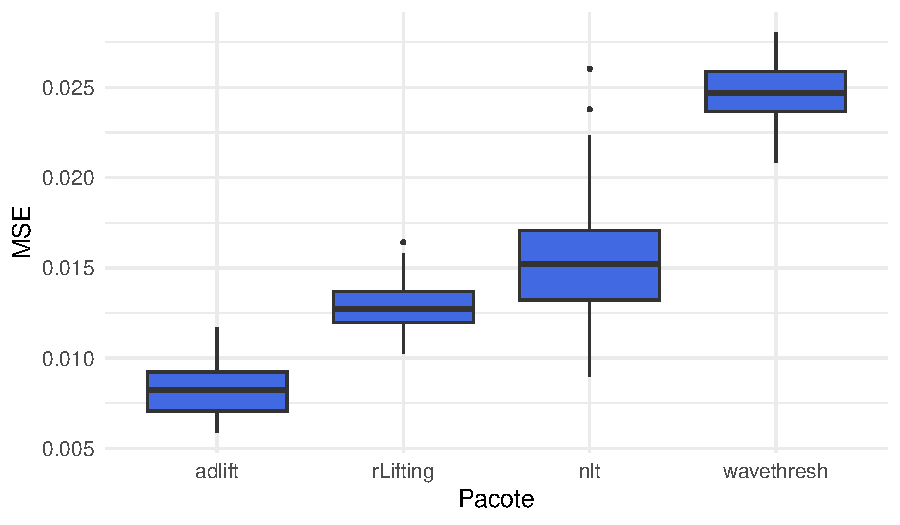
\includegraphics[width=0.75\textwidth]{figuras/benchmark_mse.pdf}
    \caption{MSE mediano na melhor configuração de cada pacote, por sinal de referência (\(T=1024\), grade regular, 1000 replicações de Monte Carlo). Menores valores indicam melhor desempenho.}
    \label{fig:rlifting-benchmark-mse}
\end{figure}

Por fim, demonstramos a capacidade de processamento em tempo real na Figura \ref{fig:realtime-denoising}. 
Nela, simulamos um fluxo contínuo de dados ruidosos (uma senoide com ruído) sendo processado ponto a ponto pelo \texttt{new\_wavelet\_stream}. 
A cada nova observação, o algoritmo atualiza a estimativa instantânea (linha azul) em tempo constante, sem acesso a dados futuros. 
O resultado evidencia que o pacote consegue recuperar a tendência subjacente do sinal (linha tracejada) com pouco atraso, viabilizando seu uso em sistemas de monitoramento \emph{online}.

\begin{figure}[H]
    \centering
    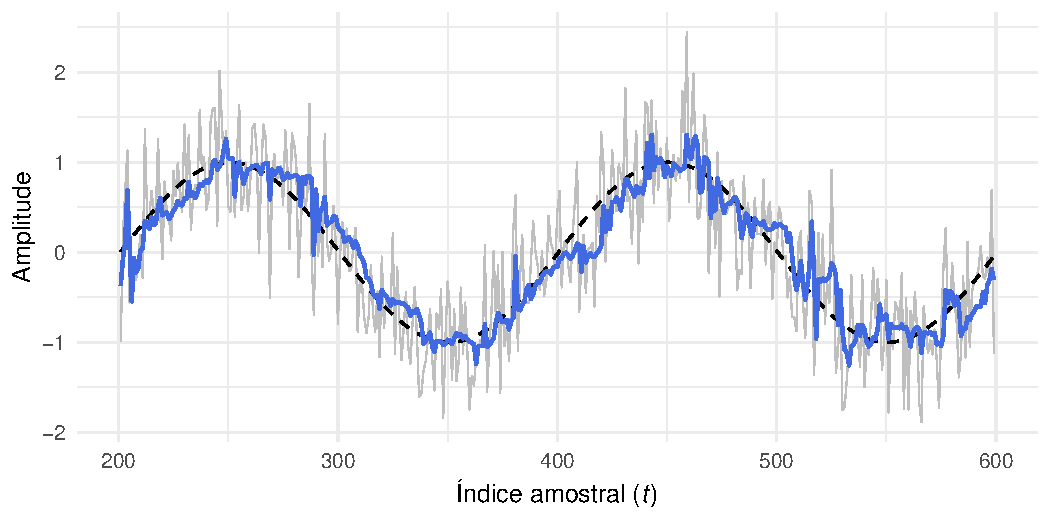
\includegraphics[width=0.75\textwidth]{figuras/realtime_denoising.pdf}
    \caption{Suavização em tempo real de um fluxo de dados. A linha sólida (azul) representa a estimativa calculada incrementalmente pelo \texttt{rLifting} à medida que novos pontos (cinza) são observados. A linha preta tracejada é a função original.}
    \label{fig:realtime-denoising}
\end{figure}

Esses resultados reforçam que o \texttt{rLifting} ocupa um nicho distinto ao oferecer a velocidade necessária para aplicações intensivas ou de tempo real, mantendo uma qualidade de reconstrução comparável às implementações já existentes da DWT.

\section{Considerações práticas de implementação}\label{sec-metodologia-consideracoes}
Nesta seção, discutimos algumas das escolhas paramétricas e limitações imediatas da nossa proposta metodológica que influenciam o desenho dos experimentos apresentados no Capítulo \ref{sec-estudos-simulacao}. 
Adiantamos que retomaremos a discussão de limitações mais fundamentais no Capítulo \ref{sec-conclusao}.

O primeiro ponto de ponderação para um analista no procedimento operacionalmente causal é a escolha do tamanho da janela móvel, \(W\). 
Janelas curtas irão reagir rapidamente a mudanças de regime no tempo real, mas limitam o nível de resolução máximo da DWT e podem inviabilizar a detecção de tendências de longo prazo. 
Uma janela excessivamente longa, todavia, faz com que a DWT \emph{online} aproxime-se de sua contraparte \emph{offline}, com a restrição, porém, de que as primeiras \(W\) observações do sinal retornado ainda estarão contaminadas pelo ruído. 
Como recomendação geral, é uma boa prática verificar informações disponíveis sobre o tamanho total do sinal, se possível, antes de determinar \(W\).

Problema similar acomete as escolhas dos hiperparâmetros \(\alpha\) e \(\beta\). 
Os valores padrão funcionam bem para uma gama de funções, mas o algoritmo pode desempenhar melhor com uma calibração mais cuidadosa. 
Para análises \emph{offline} ou em lote, a função \texttt{tune\_alpha\_beta()} seleciona \(\alpha\) e \(\beta\) minimizando o SURE sobre uma grade de parâmetros com refinamento via Nelder-Mead. 
O custo computacional é da ordem de segundos para \(T \sim 10^3\), o que a torna inviável para aplicações em tempo real estrito. 
Uma via alternativa é \texttt{threshold\_method = "sure"}, que contorna \(\alpha\) e \(\beta\) por completo, calibrando cada nível de resolução individualmente via SURE sem recorrer à recursão paramétrica. 
Em processamento por janela, o parâmetro \texttt{update\_freq} completa esse quadro ao controlar com que frequência os limiares são recalculados. 
O padrão, recálculo a cada nova amostra, maximiza a adaptabilidade, mas valores maiores reduzem o custo computacional em cenários de dados volumosos.

Ainda em relação ao \texttt{rLifting}, métodos de pré-processamento \emph{online} invariavelmente apresentam atraso de borda. 
Para procedimentos em que a causalidade operacional é necessária, recomendamos fortemente o uso de filtros mais curtos (como Haar e Daubechies 2). 
Filtros como CDF 9/7 exigem que mais pontos sejam artificialmente inseridos pela extensão de borda, o que pode comprometer a reconstrução da função subjacente. 
Este é um tópico especialmente relevante para a estimação do \(\mathrm{FATE}\), uma vez que são precisamente os pontos de borda que alimentam a regressão via mínimos quadrados nos procedimentos \emph{online}. 
O leitor há de notar que em nossas simulações fomos precavidos em relação a essa problemática.

Finalmente, conquanto seja possível construir as bandas de confiança para fluxos de estimação operacionalmente causais em cenários que não exijam a velocidade de atualizações instantâneas, gostaríamos de reiterar a impossibilidade computacional de obtenção dessas bandas para aplicações em tempo real estrito. 
Como paliativo, para estes casos mais complexos computacionalmente, sugerimos uma atualização periódica das bandas. 
Reconhecemos que essa estratégia introduz um atraso entre a obtenção dos resultados pontuais e das bandas de confiança, mas acreditamos que estes, a depender do problema, seriam toleráveis: se o fluxo de dados for alto (rápida atualização de dados), rapidamente teríamos pontos amostrais suficientes para os procedimentos de reamostragem. 
Embora a latência exista, não tardaria até que pudéssemos identificar falhas no modelo; se, por outro lado, o fluxo de dados for lento, teríamos tempo suficiente para executar o \emph{bootstrap}, efetivamente eliminando o atraso entre estimativas pontuais e intervalares.